\documentclass[12pt]{article}

\usepackage{booktabs}
\usepackage{tabularx}
\usepackage{hyperref}
\usepackage{enumitem}
\usepackage{biblatex}
\usepackage{graphicx}
\usepackage{xcolor}
\usepackage{ulem}
\usepackage{gensymb}


\addbibresource{reference.bib}
\graphicspath{./}
\hypersetup{
    bookmarks=true,         % show bookmarks bar?
      colorlinks=true,      % false: boxed links; true: colored links
    linkcolor=red,          % color of internal links (change box color with linkbordercolor)
    citecolor=green,        % color of links to bibliography
    filecolor=magenta,      % color of file links
    urlcolor=cyan           % color of external links
}

\newcommand{\lips}{\textit{Insert your content here.}}

%% Comments

\usepackage{color}

\newif\ifcomments\commentstrue %displays comments
%\newif\ifcomments\commentsfalse %so that comments do not display

\ifcomments
\newcommand{\authornote}[3]{\textcolor{#1}{[#3 ---#2]}}
\newcommand{\todo}[1]{\textcolor{red}{[TODO: #1]}}
\else
\newcommand{\authornote}[3]{}
\newcommand{\todo}[1]{}
\fi

\newcommand{\wss}[1]{\authornote{blue}{SS}{#1}} 
\newcommand{\plt}[1]{\authornote{magenta}{TPLT}{#1}} %For explanation of the template
\newcommand{\an}[1]{\authornote{cyan}{Author}{#1}}

%% Common Parts

\newcommand{\progname}{SFWRENG 4G06 Capstone Design Project} % PUT YOUR PROGRAM NAME HERE
\newcommand{\projname}{MotionMingle} % project name
\newcommand{\authname}{Team \#18, InfiniView-AI
\\ Anhao Jiao
\\ Kehao Huang
\\ Qianlin Chen
\\ Shu Qi
\\ Xunzhou Ye
} % AUTHOR NAMES

\usepackage{hyperref}
    \hypersetup{colorlinks=true, linkcolor=blue, citecolor=blue, filecolor=blue,
                urlcolor=blue, unicode=false}
    \urlstyle{same}


\begin{document}

\title{Software Requirements Specification for \progname: MotionMingle} 
\author{\authname}
\date{\today}
	
\maketitle

~\newpage

\pagenumbering{arabic}

\tableofcontents

~\newpage

\begin{table}[hp]
  \caption{Revision History} \label{TblRevisionHistory}
  \begin{tabularx}{\textwidth}{llX}
    \toprule
    \textbf{Date} & \textbf{Developer(s)} & \textbf{Change}\\
    \midrule
    25 September 2023 & AJ, KH, QC, QS, XY & Initial draft \\
    02 February 2024 & AJ, KH, QC, QS, XY & rev 0.1 \\
    22 March 2024 & AJ, KH, QC, QS, XY & rev 1 \\
    \bottomrule
  \end{tabularx}
\end{table}

~\\

~\newpage
\section{Introduction}
This document serves as a comprehensive requirements specification for a \sout{WebRTC-based video conferencing} \textcolor{red}{Real-Time video streaming} application tailored specifically for Tai Chi instruction. The purpose of this document is to provide a detailed guide for the development and implementation of the system, ensuring that all stakeholders and developers have a clear and unified understanding of the project’s scope, objectives, and functional and non-functional requirements. This document follows a structured format of the Meyer’s template, which has four major dimensions or PEGS: Project, Environment, Goals, System. The four dimensions correspond to the four major sections in this document. Slight modifications are made on the document structure to better fit our project:
\begin{itemize}
  \item The Functionality section under the System dimension is divided into the functional requirements section and the non-functional requirements section for better clarity.
  \item Added the Use Case Diagram section to illustrate use cases.
  \item Added the Finite State Machine section to provide formal specification.
\end{itemize}
\subsection{Glossary}\label{Glossary}
\begin{description}
    \item[Tai Chi] A classical Chinese martial art system practiced for health promotion and rehabilitation.
    \item[Instructor] A person who teaches a Tai Chi class through an online conference system.
    \item[Practitioner] A person who learns Tai Chi through an online conference system.
    \item[Skeleton Annotation] A type of annotation that the system can generate. This type of annotation looks like a human skeleton.
    \item\sout{\textbf{Clock Annotation}} A type of annotation that the system can generate. This type of annotation looks like a physical clock surrounding the instructor.
    \item[Center of Mass Visualization] A type of annotation that the application generates. This type of annotation shows the instructor’s center of mass with the instructor's face and feet's direction.
    \item[Semantic Segmentation] The process of linking each pixel in an image to a class label. It is a pixel-wise classification task that assigns a semantic label like “person”, “car”, “road”, etc. To every pixel in the image.
    \item[Pose Estimation/Extraction] The process of using machine learning models to estimate the pose of a person from an image or a video by estimating the spatial locations of the person’s key body joints.
    \item[2D Pose Estimation] The process of estimating the 2D position and orientation of a person or object in an image or video. This involves identifying the key points on the body or object, such as the head, shoulders, knees, etc. then estimating their position in  2D space.
    \item[3D Pose Estimation] Similar to 2D pose estimation position estimation is in 3D space. One advantage of 3D pose estimation is it can show the rotation of a body part(i.e. Wrist rotation), whereas 2D pose estimation can’t.
    \item[Machine Learning Model] A mathematical model designed to find patterns and make predictions or decisions based on data.
    \item[Server-Side Rendering]  The technique of rendering streaming video on the server instead of on clients' devices.
    \item[Annotation Pipeline] A sequence of processing elements connected in series, which are responsible for generating annotations.
    \item[Annotation Configuration] Options for practitioners to configure the annotation preference.
    \item[UI] User Interface
    \item[UX] User Experience
    \item[AI] Artificial Intelligence
    \item[OS] Operating System
    \item[\textcolor{red}{SFU}] \textcolor{red}{Selective Forwarding Unit, a component in real-time communication systems like WebRTC
    that routes and selectively forwards audio and video streams from one participant to others}
    \item[\textcolor{red}{STUN/TURN servers}] \textcolor{red}{A component in real-time communication systems that is responsible for
    establishing and maintaining connections.}
\end{description}

\subsection{\textcolor{red}{Symbolic Constants}}\label{sec:symbolic-constants}
\begin{description}
    \item[\textcolor{red}{USER\_SATISFACTION\_PERCENTAGE =}] \textcolor{red}{\%95}
    \item[\textcolor{red}{INTERNET\_UPLOAD\_SPEED =}] \textcolor{red}{5Mbps} 
    \item[\textcolor{red}{INTERNET\_DOWNLOAD\_SPEED =}] \textcolor{red}{25Mbps} 
    \item[\textcolor{red}{COMPATIBILITY\_PERCENTAGE =}] \textcolor{red}{\%95}
    \item[\textcolor{red}{LOWEST\_RESOLUTION\_SUPPORTED =}] \textcolor{red}{480P}
    \item[\textcolor{red}{HIGHEST\_RESOLUTION\_SUPPORTED =}] \textcolor{red}{1080P}
\end{description}

\section{Project}
This section provides a comprehensive overview of the project’s key aspects. It outlines the project’s structure, responsibilities of team members, technical decisions, and the plan for project execution.
\subsection{Roles and Personnel}
A team of five members is designated to carry out the planning, managing, documenting, and execution phases of the project specified in this requirements document (referred to as “the project”). The project is initiated and will be executed in the context of an accumulative academic course on software designs and life cycles. The situation presents time constraints and resource management challenges for all personnel involved. Members of the team are expected to identify potential problems that might hinder the progress of the project, voice their concerns or suggestions, acknowledge their shares of work and fulfill their own responsibilities with a high standard of quality. For each team member, the expected workload is 10 hours per week, totalling 50 hours per week. This is the typical workload of a full-time employee in the technology industry. Also constrained by the academic context, there is no preserved capacity for additional human resources. Induction of further personnel is not possible throughout the execution of the project. The project leader is expected to efficiently utilize and manage the limited resources and group members are expected to be held accountable for their duties.
\subsubsection{Individual Responsibilities}
\begin{itemize}
    \item Xunzhou Ye specializes in the machine learning portion of the project. Subsequent responsibilities include learning and investigating preliminary studies completed before the initiation of the project, and developing from and optimizing existing machine learning-powered processing pipelines. 
    \item From the managerial perspective of the project, Ye takes on the leadership role within the team. Subsequent responsibilities include envisioning the direction in which the project progresses, sustaining and/or enhancing the project momentum, coordinating team members to maintain a high level of productivity, actively listening to peer feedback, and timely stepping in and helping with resolving conflicts of interest.
    \item Qi Shu and Kehao Huang specialize in connecting and integrating machine learning with the component of the system that interfaces with the user. Subsequent responsibilities include studying the preliminary works in-depth and designing interfaces internal to the system to connect and integrate major components.
    \item From the managerial perspective, Qi is the co-project leader. Subsequent responsibilities include overseeing and documenting the progress of the project and communicating with managerial stakeholders such as academic and project supervisors.
    \item Qianlin Chen and Anhao Jiao specialize in articulating and implementing the means of interaction between the system and the end user. Subsequent responsibilities include designing the interfaces used for the communication between the system and the user and architecting both the software and hardware infrastructures to support the interfaces. 
\end{itemize}


\subsection{Imposed Technical Choices}
\textcolor{red}{N/A}
\sout{
The majority of the technical choices and decisions originate from the academic context in which the project is planned and carried out. Most of the technical resources shall be chosen from available open-source software, development tools, and intellectual assets. Despite the supervisor allotting a small budget for the completion of the project, team members shall minimize financial costs when making design choices and budgeting decisions. On the other hand, to accommodate the significant amount of computing resources required by machine learning-powered applications, our academic institution would offer computing hardware to support the operation of the specified system in the “System” book. The decision to utilize a self-hosted server, rather than opting for commercial cloud-hosted services, is clear and would help us adhere to our financial budget constraints.

Other technical choices include the choice of programming language, Python, for the machine learning component of the system, and choosing JavaScript/TypeScript for the web application component of the system. Both of these choices are rooted in the fact that the language used to describe each component aligns with industry standards and conventional practices. The technology ecosystems around the two languages are mature and well-tested.
}
\newpage
\subsection{Schedule and Milestones}
Please refer to table \ref{TblMilestones}
\begin{table}
    \caption{Milestones and Scheduled Due Dates} \label{TblMilestones}
    \begin{tabularx}{1.0\linewidth}[h]{p{7cm}|p{6cm}}
    \toprule
    \textbf{Milestone}        & \textbf{Scheduled Due Date} \\ \hline
    \midrule
    Team Formed, Project Selected                                  &   18 September 2023 \\ \hline
    Problem Statement, Proof of Concept Plan, Development Plan     &   25 September 2023 \\ \hline
    Requirements Documents Revision 0                              &   06 October 2023   \\ \hline
    Hazard Analysis Revision 0                                     &   20 October 2023   \\ \hline
    Verification and Validation Plan Revision 0                    &   03 November 2023  \\ \hline
    Proof of Concept Demonstration                                 &   Week of 17 November 2023 \\ \hline
    Design Document Revision 0                                     &   17 January 2024   \\ \hline
    Project Demonstration Revision 0                               &   Two weeks starting 05 February 2024 \\ \hline
    Verification and Validation Report Revision 0                  &   06 March 2024     \\ \hline
    Project Demonstration Revision 1 (Final)                       &   Two weeks starting 18 March 2024 \\ \hline
    Full Project Documentation Revision 1 (Final)                  &   04 April 2024 \\ \hline
    \bottomrule
    \end{tabularx}
\end{table}

\subsection{Tasks and Deliverable}
For the documentation portion for each milestone, the work shall be broken down evenly for each team member. The distribution of work shall be carefully considered. Related or connected topics shall be distributed to an individual team member. Doing so would minimize the need for frequent sync-ups with other team members. Specific division of tasks shall be brought up and discussed in the deliverables planning meetings around 2 weeks ahead of the deliverable due. The description of the divided tasks and the expected completion date shall be posted as checkbox items on the Github meeting issue.

For the implementation aspect of each milestone, there are two stages in total. The first one being to create a prototype for the proof of concept demonstration in mid-November. In this stage, the team shall be focusing on implementing the real-time video conferencing web application, which includes the user clients, UI designs, and the servicing infrastructure. At the same time, all team members shall be familiar with all technologies relevant to implementations. The second stage is to build on top of the prototype, carrying out the full implementation for the Revision 0 demonstration in February 2024. At this stage, the web application shall seamlessly integrate with the machine learning models and provide all specified functionalities and features to users.

\subsection{Required Technology Elements}
\begin{description}
\item[Programming Language:] Python JavaScript/TypeScript
\item[Linter Tool:] Flake8, ESlint
\item[Testing Framework:] \sout{pytest, Jest} \textcolor{red}{aiohttp, React Testing Library} 
\item[Code coverage:] \sout{pytest-cov, jest} \textcolor{red}{React Testing Library} 
\item[Version Contro:l] git
\item[CI/CD:] GitHub Actions
\item[Libraries:] \sout{WebRTC, PyTorch, Bun.js} \textcolor{red}{aioRTC, MediaPipe, React.js} 
\item[ML Models:] \sout{OpenPose, SMPL, ShapeMask} \textcolor{red}{MediaPipe} 
\item[UI Design framework:] \sout{Ant Design} \textcolor{red}{Material UI}
\end{description}
All of the listed tools are readily available to the public. The availability of these technology elements is crucial to the success of the project.

\subsection{Risk and Mitigation Analysis}
One potential risk for this project is insufficient background knowledge in some of the required technologies: \sout{WebRTC} \textcolor{red}{Real-Time streaming protocol}, socket programming, and computer vision. To mitigate this, time will be allocated for team members to learn these technologies before utilization in the project.

Furthermore, the current technology selections and goals may evolve over the course of development. For example, it is uncertain whether the machine learning model can generate real-time annotations given factors like network traffic and chosen server-side rendering techniques. If significant changes occur, documentation will be updated accordingly to reflect implemented adjustments.

Another potential risk affecting our project's deliverables pertains to human factors. Given that team members are concurrently engaged in multiple other courses and possess diverse life priorities, the project's progress heavily relies on effective time management among team members. It is conceivable that our pace may decelerate during peak examination periods. To mitigate this, the team collectively agreed that each member should allocate a minimum of 10 hours per week to ensure consistent progress.

Ineffective communication could also pose a risk. To minimize miscommunications, the team will hold two scheduled meetings per week, along with preparation sessions before external stakeholder meetings to ensure every team member is on the same page. Platforms such as Discord and Teams will be used for daily communication and to clarify any misunderstandings.

Finally, this project presents not just technical challenges but also demands meticulous documentation of all development processes. Meeting both objectives within the given timeframe may prove infeasible. As discussed with the course instructor, documentation will take priority if such resource conflicts arise.

\subsection{Requirements Process and Report}
In the requirement elicitation process, project requirements will be acquired during our bi-weekly meetings with the supervisor. To facilitate efficient communication and effective elicitation, it is imperative to conduct brief question preparation sessions beforehand. Additionally, as the project progresses, a clearer distinction between our project implementation and objectives will emerge. This differentiation is likely to engender new project requirements, which will be systematically identified, summarized, and incorporated into our project documentation.

\section{Environment}
% Glossary refer
\subsection{Glossary}
Please refer to \ref*{Glossary} Glossary

\subsection{Components}

\subsubsection{Hardware Components}
\begin{description}
    \item[Webcam] A Webcam is required for the instructor's client.
    \item[\sout{Microphone}] \sout{Microphone is optional for both the instructors and the practitioners.}
    \item[Monitor] A monitor is required for practitioners.
    \item[Host Server] A host server is required for routing, processing video streams and annotation generation.
    \item[Network Connection] Having access to the internet is required for both instructors and practitioners.
\end{description}
\subsubsection{Software Components}
\begin{description}
    \item[OS] The OS that the application runs on might affect the usability of the application. (i.e. the application doesn’t run on some OS)
    \item[Docker] Required for standardized application deployment from the developer’s machine to the host server.
    \item[Machine Learning Models] Machine Learning Models are required for instructor’s pose extraction.
\end{description}

\subsection{Constraints}
\begin{description}
    \item[Bandwidth] The Application must not occupy more than\\ \sout{20MB/s}\hyperref[sec:symbolic-constants]{\textcolor{red}{INTERNET\_DOWNLOAD\_SPEED}} download speed\cite{downloadSpeed2018} and \sout{5 MB/s}\hyperref[sec:symbolic-constants]{\textcolor{red}{INTERNET\_UPLOAD\_SPEED}} upload speed\cite{uploadSpeed2021}, as these two numbers are the most common home internet speeds for Canadian families.
    \item[Compatibility] The product must be able to operate on all Windows, Mac OS and Linux platforms because over \sout{95\%} 
    \hyperref[sec:symbolic-constants]{\textcolor{red}{COMPATIBILITY\_PERCENTAGE}} of the computers run on these three systems\cite{OSMarketShare}.
    \item[Security] Data leak in any video conference system is not permitted, according to the Personal Information Protection and Electronic Documents Act\cite{Law1}.
    \item[Ease of Learning] One of the target audiences of our system is senior people. This user group usually has some difficulties in using software as they have lower technical device adoption\cite{olderAdultsTechUse}. The UI interaction must be clear and intuitive enough for senior people to learn all the features without further instructions.
    \item[Compliance] The application is required to comply with all applicable laws\cite{Law1}\cite{Law2}\cite{Law3} and regulations.
\end{description}

\subsection{Assumptions}
\begin{description}
    \item[Internet Access] Users of the system are assumed to have \textcolor{red}{access to }a \sout{reliable} internet connection. Packet loss and interruptions resulting from poor network connections are \sout{generally not} accounted for.
    \item[Device Capability and Compatibility] The system is assumed to run on modern portable/non-portable computing devices with adequate computational power and basic networking and real-time data streaming capabilities. The software runtime environment on top of the capable hardware is also assumed to be up-to-date. Extensive backward compatibility with outdated, deprecated hardware or software is not required.
    \item[Understanding of the Annotation] After adding annotations to the instructor’s streaming video, practitioners are assumed to understand these annotations.
    \item[Cognitive Ability] Assume users are able to understand and use the interface of the system, presuppose that users can navigate, process information, and make informed decisions within the interface without struggling.
    \item[Supported Video Resolutions] Most users’ built-in webcams in laptops and phones are assumed to support video resolution\\ \hyperref[sec:symbolic-constants]{\textcolor{red}{LOWEST\_RESOLUTION\_SUPPORTED}} \sout{up} to \\\sout{1080p}\hyperref[sec:symbolic-constants]{\textcolor{red}{HIGHEST\_RESOLUTION\_SUPPORTED}}, which is commonly used for streaming and daily uses.
    \item[Scalability of the System] The system will be designed with scalability in mind, assuming a growing user base.
\end{description}

\subsection{Effects}
\subsubsection{Improved Online Tai Chi Instruction Quality}
By providing visual annotations, the system improves the clarity and effectiveness of online Tai Chi instruction. Instructors can convey movements more clearly, leading to better learning outcomes for practitioners.
\subsubsection{Increased Accessibility to Tai Chi}
By minimizing hardware requirements and providing an intuitive user interface, the system enables individuals who may not have access to traditional Tai Chi classes or specialized equipment to participate in Tai Chi practice from the comfort of their homes.
\subsubsection{Increased Tai Chi Awareness}
By making Tai Chi accessible to a wider audience, the platform can raise awareness about the benefits of Tai Chi, potentially leading to increased interest in and participation in Tai Chi practice in society.
\subsubsection{Reduced Carbon Footprint}
By offering Tai Chi lessons online, practitioners can practice from their own homes, reducing the need for travel to physical locations. This can result in fewer carbon emissions associated with transportation.

\subsection{Invariants}
\begin{description}
    \item[Camera] The camera used by the instructor during Tai Chi sessions must remain active and operational for the entire duration of the session.
    \item[Internet Bandwidth] Sufficient internet bandwidth for both the instructor and participants must be consistently available to maintain the quality and reliability of Tai Chi sessions.
    \item[Data Encryption] Throughout the streaming lesson, it is imperative to consistently uphold and ensure the secure transmission of user data and video call content to safeguard user privacy.
    \item[Video Transmission] The video information transmitted to the client remains invariant with respect to the source video, excluding any annotations. In other words, annotations only supplement the original content with additional information and should not alter the amount of information or the quality provided by the original videos.
\end{description}

\section{Goals}
This section outlines the goals and objectives of the project, providing context for its development. It also presents the expected benefits of the project and offers a high-level overview of the system’s functionality, limitations, and stakeholders involved in the project.
\subsection{Context and Overall Objective}
The prevailing situation in Tai Chi instruction involves a transition from traditional in-person classes to online training sessions induced by the enforcement of social distancing during the COVID-19 pandemic. The transition has imposed numerous challenges for both instructors and practitioners. This project aims to address the pressing need for an enhanced online learning platform for Tai Chi. By providing real-time annotations, minimizing hardware requirements, ensuring data security, and offering user-friendly interfaces, our project is expected to elevate online Tai Chi instruction to a smooth and enriching experience. The project is subsequently decomposed into two major components: the video conferencing platform that supports video and audio communications, and the machine learning pipelines that process the video stream from instructors and generate real-time annotations.

\subsection{Current Situation}
During the COVID-19 pandemic, group exercise classes like Tai Chi transitioned to the online format due to the enforcement of social distancing. Currently, virtual Tai Chi training is usually conducted by either offering live sessions with webcams or watching pre-recorded videos. Both ways of virtual Tai Chi training fall short compared to traditional in-person instruction as widely perceived among Tai Chi practitioners and instructors for several reasons. One significant drawback of learning Tai Chi Online is that practitioners may not be able to see all the angles of the instructor’s body needed to understand and mimic the movements. Also, the lack of real-time feedback from instructors and interaction among participants is also limiting the learning outcomes and engagement for practitioners. Therefore, the virtual Tai Chi training model is considered inferior to the traditional in-person teaching model.

\subsection{Expected Benefits}
The successful execution of the project promises several business benefits. First, it will significantly elevate the learning and teaching experience for online Tai Chi training sessions. By providing a video conferencing platform that supports real-time audio and video communication, along with offering various user-configurable annotations that enhance the visibility of the instructor’s movements, our solution aims to bridge the gap between traditional in-person instruction and the online learning model. This enhancement is expected to result in higher engagement levels and improved learning outcomes of online Tai Chi training.

Secondly, the project emphasizes the safety of user data, ensuring trust and privacy among users. By safeguarding user data and preventing any case of data leakage, the application aims to provide a secure and reliable platform for Tai Chi instructors and practitioners.

Third, the application aims to minimize the hardware requirements for end users. Ideally, the application should be accessible to users as long as they have a device that supports video conferences and has access to the internet. Therefore, the application is accessible to audiences who have an interest in learning Tai Chi online but only have digital devices with limited computing power.

Lastly, the system’s ease of use will make Tai Chi accessible to individuals of all age groups. This application should be intuitive enough to use for all users that no further instruction is required. The inclusiveness of this application not only promotes the practice of Tai Chi but also contributes to the overall well-being of individuals, aligning with the broader mission of health promotion and rehabilitation associated with Tai Chi.

To conclude, the successful execution of the proposed project is foreseen to revolutionize the landscape of virtual Tai Chi training, making it a more efficient, accessible and enriching experience for both practitioners and instructors.

\subsection{Functionality Overview}
The system is designed with multiple features tailored for practitioners. First, it ensures seamless video streaming, allowing users to watch and follow videos in real-time. Additionally, practitioners have the flexibility to select and view specific annotations on the video, which provide supplementary information or guidance. A standout capability of this system is its automated motion detection feature. This means that when the instructor's movements are detected, relevant annotations are automatically overlaid onto the video, aiding practitioners in better understanding and mirroring the demonstrated actions.
\subsection{High-Level Usage Scenarios}
For high-level usage scenarios, the system can be utilized for various purposes. The primary intended usage scenario is supporting Tai Chi teaching and learning sessions in a synchronous setting. Body movements and forms demonstrated by a Tai Chi instructor are captured in an ordinary media stream and then live-streamed to all interested practitioners. Features of the movements and forms are extracted from the media stream and used to achieve or aid in achieving the functionalities described above.

Furthermore, such a video could be extended to more generic usage scenarios. Virtually any online media conference or offline instructional record which involves showcasing and placing emphasis on human limb movements, and is created for demonstrative and educational purposes, could benefit from the additional information provided by the generated annotations. Specific examples of the use cases include but are not limited to group or personal gym workout sessions, breakdowns of movements and techniques in various sports, and demonstrations of physiotherapy or rehabilitation exercises. Finally, it has the potential to perform motion tracking, pose estimation, and body auto-rigging solely with video data input.

\subsection{Limitations and Exclusions}
The system is tailored with specific guidelines in mind. It's worth noting that the product is specially crafted to analyze and provide insights on slow movements, much like those found in Tai Chi practices. As such, it might not deliver optimal results for fast-paced or dynamic actions. There's no user login mechanism because it's deemed unnecessary for the system's core functionality. Furthermore, the feedback and instruction are designed to be general, encompassing various Tai Chi techniques without the need to segregate them into different classes. Lastly, the system focuses on providing real-time and interactive guidance, it is not compatible with video playback features.

\subsection{Stakeholders and Requirements Sources}
\subsubsection{Stakeholders}
\begin{description}
    \item[Tai Chi Practitioners] Individuals who practice Tai Chi and can benefit from real-time instruction video after model rendering.
    \item[Tai Chi Instructors] Professionals who teach Tai Chi and can utilize the system for synchronous teaching sessions.
    \item[Tai Chi Potential Practitioners] Individuals who are learning Tai Chi and can use the system to improve their practice.
    \item[Capstone Project Supervisor] A supervisor who supervises the progress of the project.
\end{description}
\subsubsection{People Other Than Stakeholders}
\begin{description}
    \item[Capstone Course Instructor] The instructor who oversees the capstone project and provides guidance and evaluation.
    \item[Course Teaching Assistants] Teaching assistants who support the capstone course and may provide additional guidance or feedback.
    \item[Capstone Project Peer Reviewers] Individuals who review and provide feedback on the capstone project.
\end{description}

\subsubsection{Predating Documentations}
There are two primary documents that predate the current research. The first encompasses feedback from users who faced challenges with plain video calls during the COVID-19 user preferences and opinions regarding annotation methods and features. The second compiles feedback from demo studies and focus groups, shedding light on user preferences and opinions regarding annotation methods and features. Together, these feedback sources offer a comprehensive view of user needs and project requirements. 

\section{System}
This section provides a detailed breakdown of the system’s desired functionalities and behavior with priorities, proposes a high-level verification plan with acceptance criteria, and states all the likely and unlikely changes of the system.
\subsection{Components}
\subsubsection{Front-End (Client-Side)}
\begin{itemize}
    \item User Interface (UI)
    \item \sout{WebRTC} \textcolor{red}{Real-Time Communication} Client
    \item \sout{Real-Time Communication Engine}
\end{itemize}
\subsubsection{Back-End (Server-Side)}
\begin{itemize}
    \item Signaling Server
    \item Selective Forwarding Unit(SFU)
    \item STUN/TURN Servers:
        \begin{itemize}
            \item STUN: Session Traversal Utilities for NAT
            \item TURN: Traversal Using Relays around NAT
        \end{itemize}
    \item API Server
    \item Machine Learning Models (Annotations)
\end{itemize}
\subsubsection{Infrastructure}
\begin{itemize}
    \item Networking
    \item Cloud
\end{itemize}
For the \sout{WebRTC-based video conferencing} \textcolor{red} {Real-Time video streaming} application using an SFU architecture, participants initiate sessions through a user interface. The \sout{WebRTC} \textcolor{red}{Real-Time Communication} Client, aided by STUN and TURN servers, manages connection establishment and multi-media stream transmissions. Real-time Communication Engine establishes, maintains, and terminates the real-time sessions. Session setup details, communicated via the Signaling Server using the Session Description Protocol (SDP), determine the following media rendering. During the video conference, the Selective Forwarding Unit (SFU) routes and optimizes media stream distribution to participants. The video streams will be extracted from the SFU server,  and transferred to the API server by the socket. Then the API server will assign its integrated Machine Learning Models to render the video and send it back to the client side. The underlying infrastructure ensures efficient data transmission, maintaining overall application performance.

\subsection{Finite State Machine}
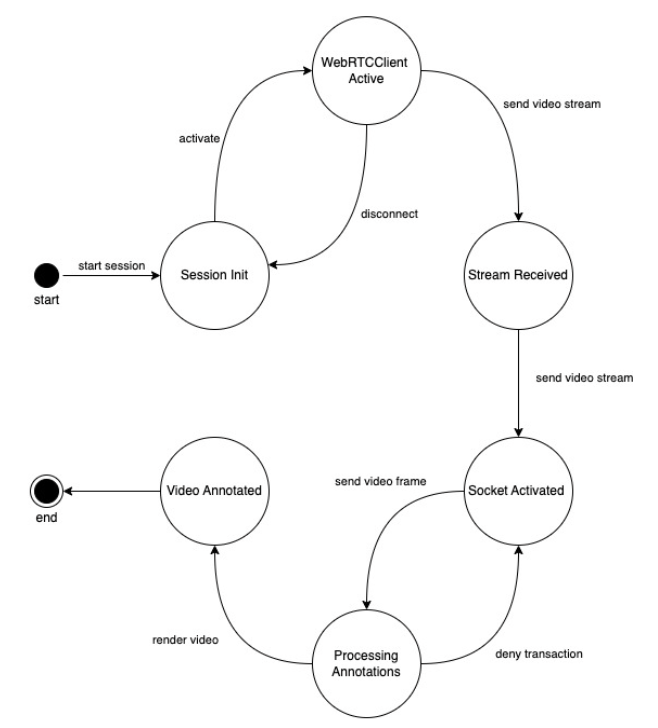
\includegraphics[width=15cm, height=7cm]{FSM.png}

\subsection{Functional Requirements}
\begin{itemize}
    \item[FR1] The system shall provide a real-time video streaming interface for Tai Chi instructors to conduct live sessions. \label{FR1}
    \begin{itemize}
        \item Rationale: This functionality allows instructors to deliver live Tai Chi classes to practitioners, facilitating real-time interaction and instruction.
        \item Priority: Critical
    \end{itemize}
\end{itemize}
\begin{itemize}
    \item[FR2] The system shall provide a real-time video streaming interface for Tai Chi practitioners to watch live sessions. \label{FR2}
    \begin{itemize}
        \item Rationale: This functionality allows practitioners to receive live Tai Chi sessions.
        \item Priority: Critical
    \end{itemize}
\end{itemize}
\begin{itemize}
    \item[FR3] The system shall turn on the webcam on the instructor’s device. \label{FR3}
    \begin{itemize}
        \item Rationale: The system needs the video stream from the instructor’s device as input.
        \item Priority: Critical
    \end{itemize}
\end{itemize}
\begin{itemize}
    \item[FR4] The system shall establish a connection between the instructor and the server. \label{FR4}
    \begin{itemize}
        \item Rationale: The system needs instructor-server connections to transmit the video and/or audio streams.
        \item Priority: Critical
    \end{itemize}
\end{itemize}
\begin{itemize}
    \item[FR5] The system shall establish the connection between each practitioner and the server for downstream data transmission. \label{FR5}
    \begin{itemize}
        \item Rationale: The system needs practitioner-server connections to transmit video and/or audio streams.
        \item Priority: Critical
    \end{itemize}
\end{itemize}
\begin{itemize}
    \item[FR6] The system shall allow practitioners to configure the type of annotations. \label{FR6}
    \begin{itemize}
        \item Rationale: The system needs user configuration details from practitioners as parameters to arrange the corresponding machine-learning pipeline.
        \item Priority: Critical
    \end{itemize}
\end{itemize}
\begin{itemize}
    \item[FR7] The system shall listen to any update on annotation configurations from practitioners. \label{FR7}
    \begin{itemize}
        \item Rationale: The server needs to update and rearrange machine learning pipelines according to annotation configurations.
        \item Priority: Critical
    \end{itemize}
\end{itemize}
\begin{itemize}
    \item[FR8] The system shall send the annotation configuration info from the practitioner-client to the server. \label{FR8}
    \begin{itemize}
        \item Rationale: The server needs to receive annotation configurations from clients.
        \item Priority: Critical
    \end{itemize}
\end{itemize}
\begin{itemize}
    \item[FR9] The system shall process the annotation configuration received from the practitioner-client. \label{FR9}
    \begin{itemize}
        \item Rationale: The system needs user configuration details from practitioners as parameters to create the corresponding machine-learning pipeline.
        \item Priority: Critical
    \end{itemize}
\end{itemize}
\begin{itemize}
    \item[FR10] The system shall arrange \sout{machine learning} \textcolor{red}{annotation} pipeline(s) based on annotation configuration. \label{FR10}
    \begin{itemize}
        \item Rationale: The system needs to generate correct annotations with the pipeline according to the practitioner’s configuration.
        \item Priority: High
    \end{itemize}
\end{itemize}
\begin{itemize}
    \item[FR11] The system shall render the instructor’s video stream with correct annotation \sout{through machine learning pipelines}. \label{FR11}
    \begin{itemize}
        \item Rationale: This is one of the outputs of the system.
        \item Priority: Critical
    \end{itemize}
\end{itemize}
\begin{itemize}
    \item[FR12] The system shall transmit the annotated video stream to each practitioner-client through an established practitioner-server connection. \label{FR12}
    \begin{itemize}
        \item Rationale: This is one of the outputs of the system.
        \item Priority: Critical
    \end{itemize}
\end{itemize}
\begin{itemize}
    \item[FR13] The signaling server shall always be available to establish \sout{WebRTC} \textcolor{red}{Real-Time streaming} connections. \label{FR13}
    \begin{itemize}
        \item Rationale: Signaling is essential for establishing real-time communications.
        \item Priority: Critical
    \end{itemize}
\end{itemize}
\begin{itemize}
\color{red}
    \item[FR14] The system shall provide 2D Pose Estimation skeleton annotation.\label{FR14}
    \begin{itemize}
        \item Rationale: Increase Tai Chi learning experience by providing the instructor's 2D Pose Estimation skeleton annotation.
        \item Priority: Critical
    \end{itemize}
\end{itemize}
\begin{itemize}
\color{red}
    \item[FR15] The system shall provide 3D Pose Estimation skeleton annotation.  \label{FR15}
    \begin{itemize}
        \item Rationale: Increase Tai Chi learning experience by providing the instructor's 3D Pose Estimation skeleton annotation.
        \item Priority: High
    \end{itemize}
\end{itemize}
\begin{itemize}
\color{red}
    \item[FR16] The system shall provide semantic segmentation annotation.  \label{FR16}
    \begin{itemize}
        \item Rationale: To distinguish the instructor from the background and make the annotation more accurate.
        \item Priority: Critical
    \end{itemize}
\end{itemize}
\begin{itemize}
    \color{red}
        \item[FR17] The system shall provide footwork annotation.  \label{FR17}
        \begin{itemize}
            \item Rationale: To identify the instructor's footwork annotation and increase Tai Chi learning experience.
            \item Priority: Critical
        \end{itemize}
    \end{itemize}
\subsection{Non-Functional Requirements}

\subsubsection{Look and Reel Requirement}
\begin{itemize}
    \item[LF1] The system shall have a user interface design that prioritizes clear and logically organized menus \label{LF1}
    \begin{itemize}
        \item Rationale: To ensure that users can comfortably use the system.
        \item Fit Criteria: \sout{95\%} \hyperref[sec:symbolic-constants]{\textcolor{red}{USER\_SATISFACTION\_PERCENTAGE}} of users are satisfied with the appearance of the UI interface.
        \item Priority: Medium
    \end{itemize}
\end{itemize}
\subsubsection{Usability and Humanity Requirement}
\textbf{Ease of Use Requirement:}
\begin{itemize}
    \item[UH1] \sout{The system shall have a straightforward and intuitive user interface design.}
    \textcolor{red}{At least \sout{90\%} \textcolor{red}{USER\_SATISFACTION\_PERCENTAGE} of the users can complete all operations and nevigation without assistance} \label{UH1}
    \begin{itemize}
        \item Rationale: To minimize user frustration and ensure a positive user experience.
        \item Fit Criteria: Users can complete common tasks within the system without extensive assistance.
        \item Priority: Medium
    \end{itemize}
\end{itemize}
\textbf{Ease of Learning Requirement}
\begin{itemize}
    \item[UH2] The system shall be easy to learn for users of all age groups and experience levels. \label{UH2}
    \begin{itemize}
        \item Rationale: To accommodate a diverse user base, including older individuals who may be less familiar with technology.
        \item Fit Criteria: Elder users can perform basic tasks and navigate the system effectively \sout{after a short learning period}
        \textcolor{red}{within 10 minutes}.
        \item Priority: Medium
    \end{itemize}
\end{itemize}
\subsubsection{Performance Requirements}
\textbf{Speed Requirement}
\begin{itemize}
    \item[PR1] The system shall respond to user interactions (e.g. button clicks, menu selections) within 1 second. \label{PR1}
    \begin{itemize}
        \item Rationale: To provide a responsive and smooth user experience.
        \item Fit Criteria: User interactions result in near-instantaneous system responses under typical conditions.
        \item Priority: Medium
    \end{itemize}
\end{itemize}
\textbf{Reliability and Availability Requirements}
\begin{itemize}
    \item[PR2] The signaling server, SFU, and STUN/TURN servers shall operate with high reliability, minimizing service interruptions during live sessions. \label{PR2}
    \begin{itemize}
        \item Rationale: To ensure a consistent and uninterrupted learning experience for users.
        \item Fit Criteria: Real-time communication services are always available.
        \item Priority: High
    \end{itemize}
\end{itemize}
\textbf{Capacity Requirement}
\begin{itemize}
    \item[PR3] The system shall support a minimum of 5 users using the system during peak usage periods. \label{PR3}
    \begin{itemize}
        \item Rationale: To accommodate a potentially large user base.
        \item Fit Criteria: The system can handle 5 simultaneous users without performance degradation.
        \item Priority: Medium
    \end{itemize}
\end{itemize}
\textbf{Robustness or Fault-Tolerance Requirement}
\begin{itemize}
    \item[PR4] The system shall implement zero fault tolerance with respect to user errors
    . \label{PR4}
    \begin{itemize}
        \item Rationale: It is essential that users receive appropriate feedback when errors occur to support system understandability.
        \item Fit Criteria: Warning messages indicating errors shall be displayed to the user to confirm lack of fault tolerance per the zero fault tolerance requirement.
        \item Priority: Medium
    \end{itemize}
\end{itemize}
\textbf{Scalability of Extensibility Requirement}
\begin{itemize}
    \item[\sout{PR5}] \sout{The system shall be able to add new extensions.} \label{PR5}
    \begin{itemize}
        \item \sout{Rationale: Further improvements and extensions of the system are needed.}
        \item \sout{Fit Criteria: Not applicable.}
        \item \sout{Priority: Medium}
    \end{itemize}
\end{itemize}
\begin{itemize}
    \item[PR6] The Selective Forwarding Unit (SFU) shall be scalable to accommodate an increasing number of simultaneous video streams as the user base grows. \label{PR6}
    \begin{itemize}
        \item Rationale: To support a growing user community without performance degradation.
        \item Fit Criteria: The SFU can handle a minimum of 10 simultaneous video streams during peak usage.
        \item Priority: Medium
    \end{itemize}
\end{itemize}
\subsubsection{Operational and Environmental Requirements}
\begin{itemize}
    \item[OE1] The system shall be compatible with the latest versions of Windows, Linux, and macOS operating systems. \label{OE1}
    \begin{itemize}
        \item Rationale: To ensure that users can access the platform regardless of their choice of operating system.
        \item Fit Criteria: The platform functions seamlessly on Windows, Linux, and macOS without critical issues.
        \item Priority: High
    \end{itemize}
\end{itemize}
\begin{itemize}
    \item[OE2] The system shall be compatible with commonly used web browsers, including but not limited to Chrome, Firefox, Safari, and Edge. \label{OE2}
    \begin{itemize}
        \item Rationale: To make the platform accessible to users who prefer different web browsers.
        \item Fit Criteria: The platform functions correctly on major web browsers without significant deviations in performance or appearance.
        \item Priority: High
    \end{itemize}
\end{itemize}
\begin{itemize}
    \item[OE3] The system shall run smoothly on standard personal computers or laptops equipped with a camera \sout{and optionally a microphone}. \label{OE3}
    \begin{itemize}
        \item Rationale: To minimize hardware-related barriers to using the platform.
        \item Fit Criteria: Users with standard personal computers or laptops can use the platform \sout{without significant performance issues}
        \textcolor{red}{with a video streaming latency of less than 500 ms while maintaining a minimum frame rate of 10 fps}.
        \item Priority: High
    \end{itemize}
\end{itemize}
\subsubsection{Maintainability and Support Requirements}
\begin{itemize}
    \item[MS1] The system shall be designed for ease of maintenance and updates. \label{MS1}
    \begin{itemize}
        \item Rationale: To ensure that the system can be efficiently maintained and improved over time.
        \item Fit Criteria: Updates and maintenance tasks can be performed with minimal disruption to users.
        \item Priority: Medium
    \end{itemize}
\end{itemize}
\begin{itemize}
    \item[\sout{MS2}] \sout{The system shall take no longer than 4 hours to be maintained/updated.} \label{MS2}
    \begin{itemize}
        \item \sout{Rationale: To ensure the availability of the system.}
        \item \sout{Fit Criteria: Updates can be done within 4 hours.}
        \item \sout{Priority: Low}
    \end{itemize}
\end{itemize}
\subsubsection{Security Requirements}
\begin{itemize}
    \item[\sout{SR1}] \sout{The system shall securely transmit and store user data, including personal information.} \label{SR1}
    \begin{itemize}
        \item \sout{Rationale: To protect user privacy and data integrity.}
        \item \sout{Fit Criteria: User data is encrypted both in transit and at rest, and security protocols follow industry best practices.}
        \item \sout{Priority: Critical}
    \end{itemize}
\end{itemize}
\begin{itemize}
    \item[SR2] The system shall not collect any non-essential information from users. \label{SR2}
    \begin{itemize}
        \item Rationale: This prevents unauthorized disclosure of users' information.
        \item Fit Criteria: Any information gathering requires users’ consent.
        \item Priority: Critical
    \end{itemize}
\end{itemize}
\begin{itemize}
    \item[SR3] The system shall not be able to be modified by unauthorized users. \label{SR3}
    \begin{itemize}
        \item Rationale:  This prevents the system from malfunctioning.
        \item Fit Criteria: Any updates/modifications to the system shall only be
made and reviewed by the development team.
        \item Priority: Critical
    \end{itemize}
\end{itemize}
\subsubsection{Cultural Requirements}
\begin{itemize}
    \item[CR1] The system shall not display any offensive cultural symbol/language. \label{CR1}
    \begin{itemize}
        \item Rationale: The intended users of the system are considered to have various cultural and religious backgrounds.
        \item Fit Criteria: Not applicable.
        \item Priority: Critical
    \end{itemize}
\end{itemize}
\subsubsection{Legal Requirements}
\begin{itemize}
    \item[LR1] The system shall meet the ISO/IEC 12207. \label{LR1}
    \begin{itemize}
        \item Rationale: ISO/IEC 12207 is an international standard for software lifecycle processes.
        \item Fit Criteria: The system meets the standard of ISO/IEC 12207.
        \item Priority: Critical
    \end{itemize}
\end{itemize}
\subsubsection{Health and Safety Requirements}
\begin{itemize}
    \item[HS1] The system shall not cause the computers to overload. \label{HS1}
    \begin{itemize}
        \item Rationale: The system should not overload the users’ computers.
        \item Fit Criteria: The hardware running the system is under normal temperature \textcolor{red}{65\degree C}.
        \item Priority: Medium
    \end{itemize}
\end{itemize}
\begin{itemize}
    \item[HS2] The system shall not affect users’ physical and mental health. \label{HS2}
    \begin{itemize}
        \item Rationale: The system must not harm users’ health and safety.
        \item Fit Criteria: \textcolor{red}{99\% of the} users feel comfortable using the system in various situations.
        \item Priority: Critical
    \end{itemize}
\end{itemize}

\subsection{Interfaces}
\subsubsection{Interface Provided By The System}
\begin{description}
    \item[User Interface] This is the primary medium most users will interact with and its design is based on the popular UI design pattern (like the Ant Design). Features include video display windows, control buttons (e.g. mute, camera toggle), participant lists, settings panels, etc.
\end{description}
\subsubsection{Hardware Interfaces}
\begin{description}
    \item[Camera \sout{and Microphone}] To capture video \sout{and audio} from users’ sides, the system interfaces with hardware drivers and OS-level APIs.
    \item[Network] For managing connections, the system might interact with the underlying operating system’s networking stack.
\end{description}
\subsection{Detailed Usage Scenarios}
The real-time video conference application leverages its underlying infrastructure, which includes components like the \sout{WebRTC} \textcolor{red}{Real-Time Communication} Client, SFU, and API server, to offer a seamless and enriched teaching and learning experience. The instructor's video rendered by machine learning annotations acts as a real-time guide, enhancing the practitioners' understanding and mastery of Tai Chi.

The detailed usage for the two main users, Tai Chi practitioners and instructors, is listed as follows:
\begin{itemize}
    \item Practitioners initiate their sessions through the application's user interface. Upon joining, the \sout{WebRTC} \textcolor{red}{Real-Time Communication} Client, with the assistance of STUN and TURN servers, ensures a stable connection for the participant. As they enter the session, they receive the instructor's video feed that's routed through the Selective Forwarding Unit (SFU). This media stream, having been extracted from the SFU server, is then relayed to the API server via a socket connection. The API server, having integrated annotation capabilities, renders the instructor's video by overlaying instructional annotations. This enhanced media stream, filled with real-time annotations detailing specific Tai Chi movements, is then returned to the practitioner's side. Throughout this process, practitioners have a passive role, in that they do not upload videos but solely benefit from the real-time instruction and the added value of the annotations on the instructor's video.
    \item Instructors initiate their teaching sessions via the same user interface. Their \sout{WebRTC} \textcolor{red}{Real-Time Communication} Client, in tandem with the STUN and TURN servers, establishes a connection. As instructors demonstrate Tai Chi forms and movements, their video stream is managed by the Real-time Communication Engine, passing session setup details via the Signaling Server using the Session Description Protocol (SDP). Their live video then gets channelled through the SFU, ensuring optimal distribution to all attending practitioners. Post this, the instructor's video stream undergoes a transformation at the API server where it's augmented with instructional annotations. These annotations might highlight specific postures, movement trajectories, or key focus areas, thereby enhancing the instructional value of the video. This annotated video is then disseminated in real-time to all the practitioners, ensuring they have a clear and enhanced understanding of the Tai Chi instructions being provided.
\end{itemize}
\subsection{Use Case Diagram}
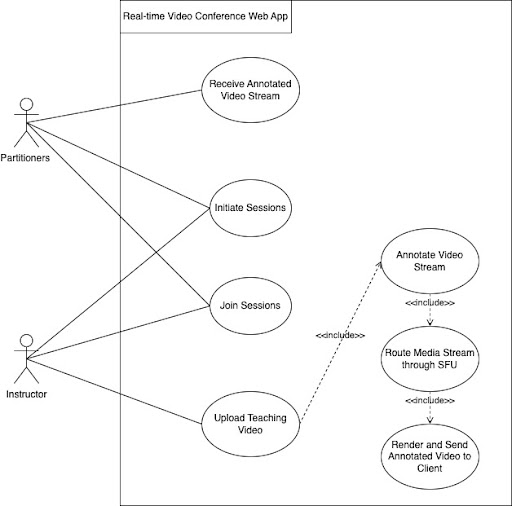
\includegraphics[width=15cm, height=15cm]{use_case_diagram.jpg}
\subsection{Prioritization}
The priorities of functionalities and behaviours are classified into four groups: Critical, high, medium and low. 
\begin{itemize}
    \item Critical:
    \begin{itemize}
        \item[] FRs: FR1 \ref{FR1}, FR2 \ref{FR2}, FR3 \ref{FR3}, FR4 \ref{FR4}, FR5 \ref{FR5}, FR6 \ref{FR6}, FR7 \ref{FR7}, FR8 \ref{FR8}, FR9 \ref{FR9}, FR11 \ref{FR11}, FR12 \ref{FR12}, FR13 \ref{FR13}
        \item[] NFRs: SR1 \ref{SR1}, SR2 \ref{SR2}, SR3 \ref{SR3}, CR \ref{CR1}, LR1 \ref{LR1}, HS2 \ref{HS2}
    \end{itemize}
    \item High:
    \begin{itemize}
        \item[] FRs: FR10 \ref{FR10}, 
        \item[] NFRs: PR2 \ref{PR2}, OE1 \ref{OE1}, OE2 \ref{OE2}, OE3 \ref{OE3}
    \end{itemize}
    \item Medium:
    \begin{itemize}
        \item[] FRs: Not applicable.
        \item[] NFRs: LF1 \ref{LF1}, UH1 \ref{UH1}, UH2 \ref{UH2}, PR1 \ref{PR1}, PR3 \ref{PR3}, PR4 \ref{PR4}, PR5 \ref{PR5}, PR6 \ref{PR6}, MS1 \ref{MS1}, HS1 \ref{HS1}
    \end{itemize}
    \item Low:
    \begin{itemize}
        \item[] FRs: Not applicable.
        \item[] NFRs: MS2 \ref{MS2}
    \end{itemize}
\end{itemize}
\subsection{Verification and Acceptance Criteria}
The high-level verification and acceptance criteria outlined below are intended to ensure that the system meets the specified requirements and presents desired behaviours.
\subsubsection{Integration of Data Streams}
\begin{itemize}
    \item Verification:
        \begin{itemize}
            \item Conduct module testing to ensure that video and audio data streams are transmitted and received without significant loss of quality.
            \item Perform system testing to verify that data streams maintain integrity during real-time communication sessions.
            \item Conduct static analysis to identify and mitigate potential issues related to data stream integrity.
        \end{itemize}
    \item Acceptance Criteria:
        \begin{itemize}
            \item Video streams should maintain a minimum resolution of 720p with minimal artifacts.
            \item Audio streams should have clear and intelligible sound quality.
            \item During system testing, no critical issues related to data stream integrity should be identified.
        \end{itemize}
\end{itemize}
\subsubsection{Accurate Response to Client Requests and Annotation Configurations}
\begin{itemize}
    \item Verification:
        \begin{itemize}
            \item Perform integration testing to ensure that the system accurately responds to client requests and annotation configurations.
            \item Conduct user acceptance testing with practitioners to validate the system’s responsiveness to annotation preferences.
        \end{itemize}
    \item Acceptance Criteria:
        \begin{itemize}
            \item The system should accurately apply annotation configurations specified by practitioners.
            \item Practitioners should confirm that their requested annotation preferences are correctly implemented during user acceptance testing.
        \end{itemize}
\end{itemize}
\subsubsection{Real-Time Processing}
\begin{itemize}
    \item Verification:
        \begin{itemize}
            \item Conduct system testing to assess the system’s ability to process video streams in real-time.
            \item Evaluate the system’s performance under various load conditions, ensuring real-time processing is maintained.
        \end{itemize}
    \item Acceptance Criteria:
        \begin{itemize}
            \item The system should consistently process video streams with minimal delay, aiming for a latency of less than 500 ms while maintaining a minimum frame rate of 10 fps.
            \item Under typical load conditions, the system should sustain real-time processing without significantly degrading the performance.
        \end{itemize}
\end{itemize}
\subsubsection{Starting/Joining Call Sessions}
\begin{itemize}
    \item Verification:
        \begin{itemize}
            \item Perform integration testing to ensure that both instructors and practitioners can start/join call sessions without encountering critical errors.
            \item Conduct user acceptance testing to assess the ease of starting/joining call sessions.
        \end{itemize}
    \item Acceptance Criteria:
        \begin{itemize}
            \item Users should be able to start/join call sessions without experiencing crashes or disruptions.
            \item User acceptance testing should confirm that the process of starting/joining a call session is straightforward and user-friendly.
        \end{itemize}
\end{itemize}
\subsubsection{Start Annotation Pipeline Based on Need}
\begin{itemize}
    \item Verification:
        \begin{itemize}
            \item Conduct module testing to verify that annotation pipelines are initiated based on practitioner preferences.
            \item Evaluate the system’s ability to dynamically start and stop annotation pipelines during live sessions.
        \end{itemize}
    \item Acceptance Criteria:
        \begin{itemize}
            \item Annotation pipelines should be initiated and terminated based on practitioner preferences.
            \item Users should have a seamless experience with annotations starting, stopping or switching as needed during live sessions.
        \end{itemize}
\end{itemize}

\subsection{Traceability Matrix}
Please refer to \ref{TblTrace_1} and \ref{TblTrace_2}.
\begin{table}[h!]
    \centering
    \begin{tabular}{|c|c|c|c|c|c|c|c|}
    \hline
        & FR1 & FR2 & FR3 & FR4 & FR5 & FR6 & FR7 \\
    \hline
    LF1 & X & X & X & & & X &   \\ \hline
    UH1 & X & X & X & & & X &   \\ \hline
    UH2 & X & X & X & & & X &   \\ \hline
    PR1 & X & X & & & & X &   \\ \hline
    PR2 & & & & X & X & &   \\ \hline
    PR3 & X & X & & X & X & &   \\ \hline
    PR4 & X & X & X & & & X &   \\ \hline
    PR5 & & & & & & &   \\ \hline
    PR6 & & & & & & &   \\ \hline
    OE1 & X & X & X & & & &   \\ \hline
    OE2 & X & X & X & & & &   \\ \hline
    OE3 & X & X & X & & & &   \\ \hline
    MS1 & X & X & X & X & X & X & X   \\ \hline
    MS2 & X & X & X & X & X & X & X   \\ \hline
    SR1 & & & & X & X & &   \\ \hline
    SR2 & X & X & & & & &   \\ \hline
    SR3 & X & X & X & X & X & X & X \\ \hline
    CR1 & X & X & & & & &   \\ \hline
    LR1 & X & X & X & X & X & X & X \\ \hline
    HS1 & X & X & & & & &   \\ \hline
    HS2 & X & X & & & & &   \\ \hline
    \end{tabular}
    \caption{Traceability Matrix Showing the Connections Between Functional Requirements and Non-functional Requirements} \label{TblTrace_1}
\end{table}

\begin{table}[h!]
    \centering
    \begin{tabular}{|c|c|c|c|c|c|c|c|}
    \hline
        & FR8 & FR9 & FR10 & FR11 & FR12 & FR13 \\
    \hline
    LF1 & & & & & &    \\ \hline
    UH1 & & & & & &    \\ \hline
    UH2 & & & & & &    \\ \hline
    PR1 & & & & & &    \\ \hline
    PR2 & & & & & & X   \\ \hline
    PR3 & & & & & X & X    \\ \hline
    PR4 & & & & & &    \\ \hline
    PR5 & & & X & & X & X    \\ \hline
    PR6 & & & X & & X & X    \\ \hline
    OE1 & & & & & &    \\ \hline
    OE2 & & & & & &    \\ \hline
    OE3 & & & & & &    \\ \hline
    MS1 & X & X & X & X & X & X  \\ \hline
    MS2 & X & X & X & X & X & X  \\ \hline
    SR1 & & & & & X & X   \\ \hline
    SR2 & & & & & &    \\ \hline
    SR3 & X & X & X & X & X & X  \\ \hline
    CR1 & & & & & &    \\ \hline
    LR1 & X & X & X & X & X & X  \\ \hline
    HS1 & & & & & &    \\ \hline
    HS2 & & & & & &    \\ \hline
    \end{tabular}
    \caption{Traceability Matrix Showing the Connections Between Functional Requirements and Non-functional Requirements} \label{TblTrace_2}
\end{table}

\newpage
\subsection{Likely/Unlikely Changes}
\subsubsection*{Likely Changes}
\begin{itemize}
  \item The application could be extended in the future to offer mobile compatibility, providing users accessibility on both desktop and mobile platforms.
  \item A login and access control system may need to be implemented to restrict video streaming capabilities to authorized users only, in order to adhere to security best practices.
  \item Additional features may need to be incorporated into future iterations based on discoveries from real-world usage and direct end user feedback.
  \item Web application compatibility may be offered to provide increased reach and usability across different devices and operating systems.
  \item The initial system load capacity will be set conservatively due to unknown demand. As user adoption increases over time, load capacity can be scaled up to support larger volumes of traffic.
  \item The Real-Time Processing requirement might change as no metric has been provided from the stakeholders.
  \item The application may be extended in the future to offer functionality to allow practitioners to stream their videos and audios.
\end{itemize}
\subsubsection*{Unlikely Changes}
\begin{itemize}
  \item The application will be designed to comply with all applicable laws and regulations\cite{Law1}\cite{Law2}\cite{Law3}. User personal information will only be collected or used with explicit consent.
  \item Given this is a student capstone project, the primary stakeholder and client is unlikely to change.
  \item As a student capstone project, schedule and budget constraints are relatively fixed and not expected to change significantly.
  \item The user input to the application and the outputs to users should remain unchanged, as the overall objective is determined.
  \item A key priority in the system design will be ease of use and learnability, given the target user base has less technical expertise.
  \item The application will implement access controls to ensure users only view data they are properly authorized to access.
  \item Annotation generation will occur in a dedicated backend system.
  \item The application will allow configurable annotation types displayed to practitioners.
  \item The application is intended to operate on Windows, Linux and MacOS platforms, but not limited to running on these systems natively.
  \item Secure data transmission and storage will be implemented to safeguard user data and mitigate data leakage risks.
\end{itemize}

\section{Appdendix}

\subsection{Reflection}

\textcolor{red}{Writing the Software Requirements Specification was a crucial phase that laid the foundational blueprint for our 
entire development process. During this stage, we delved deeply into understanding and defining the core functionalities, 
non-functional requirements, and the overall scope of our WebRTC-based video streaming application tailored for Tai Chi 
instruction. We collaboratively identified the key features necessary for a successful implementation, such as real-time 
video streaming, user-centred design, and machine learning integration for annotations. In doing so, we faced the challenge 
of translating broad concepts and goals into clear, detailed specifications that could guide our development efforts effectively.}

\textcolor{red}{One of the most significant aspects of this phase was the risk and mitigation analysis. We identified potential 
risks, such as insufficient technical knowledge in specific areas like WebRTC and real-time streaming protocols, and the 
challenge of integrating machine learning models for real-time annotations. As a team, we not only pinpointed these risks 
but also developed strategies to mitigate them, which included allocating time for learning and experimentation. Moreover, 
the process of creating the SRS reinforced the importance of clear communication and collaboration amongst ourselves. We learned 
to articulate our thoughts and ideas precisely, ensuring that every team member had a unified understanding of the project's 
objectives and requirements.}

\printbibliography

\end{document}